\begin{figure*}[t]
    \makebox[\textwidth][c]{
    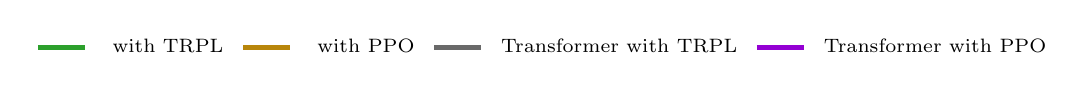
\begin{tikzpicture}
    \tikzstyle{every node}=[font=\scriptsize]
    \definecolor{tabblue}{RGB}{31, 119, 180}
\definecolor{taborange}{RGB}{255, 127, 14}
\definecolor{tabgreen}{RGB}{44, 160, 44}
\definecolor{tabred}{RGB}{214, 39, 40}
\definecolor{tabpurple}{RGB}{148, 103, 189}
\definecolor{tabbrown}{RGB}{140, 86, 75}
\definecolor{tabpink}{RGB}{227, 119, 194}
\definecolor{tabgray}{RGB}{127, 127, 127}
\definecolor{tabolive}{RGB}{188, 189, 34}
\definecolor{tabcyan}{RGB}{23, 190, 207}
\definecolor{lightblue}{RGB}{173, 216, 230}
\definecolor{sandybrown}{RGB}{244, 164, 96}
\definecolor{darkgrey}{RGB}{169, 169, 169}
\definecolor{dimgrey}{RGB}{105, 105, 105}
\definecolor{olivedrab}{RGB}{107, 142, 35}
\definecolor{darkviolet}{RGB}{148, 0, 211}
\definecolor{darkgoldenrod}{RGB}{184, 134, 11}
\definecolor{darkblue}{RGB}{0, 0, 139}
\definecolor{orchid}{RGB}{218, 112, 214}

    \begin{axis}[%
        hide axis,
        xmin=10,
        xmax=50,
        ymin=0,
        ymax=0.1,
        legend style={
            draw=white!15!black,
            legend cell align=left,
            legend columns=4,
            legend style={
                draw=none,
                column sep=1ex,
                line width=1pt,
            }
        },
        ]
        \addlegendimage{line legend, tabgreen, ultra thick} % Thicker line here
        \addlegendentry{\textbf{\model} with TRPL}
        \addlegendimage{line legend, darkgoldenrod, ultra thick} % Thicker line here
        \addlegendentry{\textbf{\model} with PPO}
        \addlegendimage{line legend, dimgrey, ultra thick} % Thicker line here
        \addlegendentry{Transformer with TRPL}
        \addlegendimage{line legend, darkviolet, ultra thick} % Thicker line here
        \addlegendentry{Transformer with PPO}
    \end{axis}
\end{tikzpicture}

    }
    \centering
    \begin{subfigure}[b]{0.32\linewidth}
        \includegraphics[width=\textwidth]{ICLR_2025/Figures/eval_ppo_3_tasks_5_seeds/smooth_eval_ppo_Isaac-Rigid-Insertion-Multi-v0_eval_consistent.pdf}
    \end{subfigure}
    \hfill
    \begin{subfigure}[b]{0.32\linewidth}
        \includegraphics[width=\textwidth]{ICLR_2025/Figures/eval_ppo_3_tasks_5_seeds/smooth_eval_ppo_Isaac-Rope-Shaping-v0_eval_all.pdf}
    \end{subfigure}
    \hfill
    \begin{subfigure}[b]{0.32\linewidth}
        \includegraphics[width=\textwidth]{ICLR_2025/Figures/eval_ppo_3_tasks_5_seeds/smooth_eval_ppo_Isaac-Cloth-Hanging-Multi-v0_eval_all.pdf}
    \end{subfigure}
    
    
    \caption{Performance comparison between HEPi and Transformer models with TRPL and PPO over 10 seeds. TRPL shows stable performance across all tasks, while PPO struggles in tasks requiring high exploration, especially in 3D environments like \textit{cloth-hanging-3D}. In tasks with a lower-dimensional action space (e.g., 2D tasks), both methods perform comparably when carefully tuned.
    % We evaluated each method over 5 seeds, performing a grid search for the best PPO parameters across an additional 5 seeds
    }
    \vspace{-0.2cm}
    \label{fig:eval_trpl_ppo}
\end{figure*}
